\documentclass{article}
\usepackage[english]{babel}
\usepackage{graphicx}
\usepackage{lipsum}
\begin{document}

\begin{figure}
    
\includegraphics[width=1\linewidth]{images/1_AUEB-pantone-HR.jpg}
\label{fig:enter-label}
\end{figure}


\title{\textbf{Time Series Forecasting and Foundation Models}}
\author{Theofanis Bakloris t8210094\\
Department of Management Science and Technology \\
Athens University of Economics and Business}
\date{July 2025}

\selectlanguage{english}
\newpage
\maketitle
\tableofcontents 

\newpage
\section{Abstract}
\title{\textbf{Time Series Forecasting and Large Language Models.}} \\
\\
This thesis explores advanced approaches to time series forecasting, with a focus on predicting visitor counts in retail stores. The study integrates both traditional deep learning techniques and cutting-edge transformer-based architectures. Initially, a neural network with Long Short-Term Memory (LSTM) layers is developed to model temporal dependencies in historical visitor data. To benchmark and extend performance, two state-of-the-art Large Language Models designed for time series forecasting are employed: Time-GPT from Nixtla and Chronos Time-LLM. These models leverage pretraining on large temporal datasets to enable accurate zero-shot and few-shot forecasting. Through evaluation, the thesis demonstrates that while the LSTM-based model captures sequential patterns well enough, more improved models like TimeGPT  significantly enhance prediction accuracy, particularly in multi-step, low-data scenarios and long forecasting horizons. The results show the growing imoprtance of pretrained time-aware language models in retail analytics and open new pathways for scalable, data-efficient forecasting systems.
This thesis explores advanced approaches to time series forecasting, with a focus on predicting visitor counts in retail stores. The study integrates both traditional deep learning techniques and cutting-edge transformer-based architectures. Initially, a neural network with Long Short-Term Memory (LSTM) layers is developed to model temporal dependencies in historical visitor data. To benchmark and extend performance, two state-of-the-art Large Language Models designed for time series forecasting are employed: Time-GPT from Nixtla and Chronos Time-LLM. These models leverage pretraining on large temporal datasets to enable accurate zero-shot and few-shot forecasting. Through evaluation, the thesis demonstrates that while the LSTM-based model captures sequential patterns well enough, more improved models like TimeGPT  significantly enhance prediction accuracy, particularly in multi-step, low-data scenarios and long forecasting horizons. The results show the growing imoprtance of pretrained zero-shot models in retail analytics and open new pathways for scalable, data-efficient forecasting systems ,that are even simplier to use.

\section{Introduction}
\subsection{Background and Motivation}
Time series forecasting is a critical component in many data-driven decision-making processes. Accurate forecasts can significantly improve operational efficiency in areas such as retail, finance, energy management, and logistics. In retail, in particular, forecasting visitor traffic allows businesses to optimize staffing, manage inventory, and enhance customer experience by aligning resources with demand patterns.\\
\\
Over the years, time series forecasting has evolved from traditional statistical methods such as ARIMA to more advanced machine learning and deep learning models. Recurrent Neural Networks (RNNs) and Long Short-Term Memory (LSTM) networks have gained popularity due to their ability to model sequential dependencies. More recently, Transformer-based models have been successfully adapted to time series tasks, with architectures such as Time-GPT and Chronos Time-LLM offering powerful alternatives by leveraging the strengths of large language models (LLMs) in sequence modeling.\\
\\
My motivation for this thesis stems from my internship, during which I worked on forecasting the number of visitors to retail stores using real-world data. I encountered various limitations in traditional models when applied to high-frequency, nonlinear visitor patterns. This experience highlighted the potential benefits of integrating pre-trained transformer models for time series forecasting and inspired the present work.

\subsection{Problem Statement}
The core objective of this thesis is to forecast the number of visitors to a retail store for the upcoming week, based on historical hourly data. The task involves multi-step forecasting, requiring the model to generate predictions for several time steps into the future.\\
\\
This problem is challenging due to ,mostly, the presence of fluctuations influenced by external factors such as holidays or promotions. Moreover, balancing forecasting accuracy with computational efficiency is essential in real-world deployments. Therefore, this thesis investigates how different models handle these challenges and compares their effectiveness across various dimensions.

\subsection{Objectives}
The main objectives of this thesis are as follows:

\begin{itemize}
    \item To implement and train a Long Short-Term Memory (LSTM) model for time series forecasting using hourly visitor data.
\end{itemize}

\begin{itemize}
    \item To apply Time-GPT in both zero-shot and fine-tuned settings and assess its suitability for long-horizon (weekly) forecasting tasks.
\end{itemize}

\begin{itemize}
    \item To evaluate the performance of the Chronos Time-LLM model, with particular attention to its architectural limitation of 64-step predictions.
\end{itemize}

\begin{itemize}
    \item To compare the forecasting accuracy of all models using as metric the Mean Absolute Error (MAE).
\end{itemize}

\begin{itemize}
    \item To visualize the forecast outputs and interpret the ability of each model to capture temporal dynamics.
\end{itemize}

\begin{itemize}
    \item To highlight the practical implications of using pre-trained large language models in operational forecasting pipelines.
\end{itemize}


\newpage
\section{Literature Review}
\subsection{Time Series Forecasting: Traditional Approaches}
Traditional time series forecasting methods rely on well-established statistical models, most notably Autoregressive Integrated Moving Average (ARIMA) and its seasonal counterpart SARIMA. These models are widely used due to their simplicity and interpretability when applied to univariate, stationary data. They model the dependencies within the time series through autoregression, differencing, and moving average terms.\\
\\
Another common approach involves Exponential Smoothing (ETS) and the Holt-Winters method, which are suitable for series with trend and seasonal components. These models emphasize recent observations and use smoothing factors to adjust level, trend, and seasonality over time. However, they rely on strong linearity assumptions and struggle when faced with nonstationarity or sudden structural changes\\
\\
More recently, tools like Facebook Prophet have been developed to make time series forecasting accessible and robust. Prophet uses an additive model combining trend, seasonality, and holiday effects, and it is particularly suited to business time series with recurring patterns and outliers. Nevertheless, Prophet shares limitations with other classical approaches in that it assumes additive components and lacks mechanisms to model complex non-linear relationships or interactions among variables\\
\\
A major limitation of these traditional models is their reliance on domain-specific preprocessing and manual tuning. They are not well-suited for high-dimensional or multivariate time series, and their performance often degrades when applied to noisy or irregular datasets. These shortcomings have prompted increased interest in machine learning approaches that can learn patterns from data automatically.

\subsection{Machine Learning in Time Series}
Machine learning (ML) techniques have gained traction in time series forecasting for their ability to model nonlinear dependencies and accommodate multivariate inputs. Unlike classical models, ML methods do not require prior assumptions about the data's distribution or structure. This makes them suitable for a broad range of forecasting tasks, especially in domains with irregular, nonstationary, or high-dimensional data.\\
\\
Among the most widely used models are Random Forests, Gradient Boosting Machines (GBMs) such as XGBoost, Support Vector Regression (SVR), and Decision Trees. These algorithms are trained on lag-based features, rolling statistics, calendar variables, and other derived features that encode time-dependent behavior. In particular, XGBoost has demonstrated strong performance in both short-term and long-term forecasting tasks due to its efficiency and ability to handle missing data.\\
\\
Despite their flexibility, machine learning models treat time series forecasting as a standard supervised regression problem. They rely heavily on feature engineering to capture temporal dynamics since they do not natively model sequential dependencies. Additionally, they often require substantial labeled data and lack built-in mechanisms for uncertainty quantification, which limits their use in risk-sensitive applications.\\
\\
As time series tasks have grown in complexity — including longer forecasting horizons, complex seasonality, and dependence on exogenous variables — researchers have turned to deep learning methods. These approaches can model sequential behavior directly and learn rich representations from raw time series data without requiring extensive feature design.

\subsection{Deep Learning for Sequential Data (RNNs, LSTMs)}
Deep learning has emerged as a powerful approach for time series forecasting due to its capacity to learn complex temporal patterns directly from raw data. Unlike classical models, which rely on manual feature engineering or statistical assumptions, deep learning models can automatically extract hierarchical and long-term dependencies through sequential architectures. Two of the most prominent neural network types for sequential modeling are Recurrent Neural Networks (RNNs) and their improved variant, Long Short-Term Memory (LSTM) networks.\\
\\
\title{\textbf{Recurrent Neural Networks}}\\
\\
RNNs are designed specifically to handle sequential input by maintaining an internal memory that captures information about previous time steps. At each time step, an RNN receives an input vector and updates a hidden state based on both the new input and the state from the previous time step. This feedback loop allows the network to build representations that are dependent on temporal order.
\\
However, RNNs face major challenges in practice. Chief among these is the vanishing gradient problem, which inhibits the network's ability to learn long-range dependencies across sequences. This issue is particularly severe when forecasting time series data with long memory effects, such as seasonal patterns or delayed responses to external variables.\\
\\
These limitations have led to the development of more robust architectures, particularly LSTMs, which introduce mechanisms to mitigate the degradation of learning across time.\\
\\
\title{\textbf{Long-Short Term Mermory Networks (LSTM)}}\\
LSTM networks were proposed by Hochreiter and Schmidhuber in 1997 as an extension of standard recurrent neural networks (RNNs), specifically designed to mitigate the vanishing gradient problem. They introduce a memory cell that can maintain information over long sequences, regulated by three gating mechanisms:

\begin{itemize}
    \item \textbf{Input gate}: controls how much new information enters the memory.
\end{itemize}

\begin{itemize}
    \item \textbf{Forget gate}: determines what information should be discarded.
\end{itemize}

\begin{itemize}
    \item \textbf{Output gate}: decides how much of the memory should be passed to the next layer.
\end{itemize}

This internal gating structure allows LSTMs to model long-term dependencies and sequential relationships in data more effectively than simple RNNs, which often fail to retain relevant temporal context beyond a few steps. \cite{garg2022machine}\\
\\
LSTMs have shown excellent performance in a wide range of time series forecasting tasks, including financial market prediction, electricity load forecasting, and retail demand forecasting. Their strength lies in their ability to process entire sequences of data, automatically learning patterns such as trend, seasonality, and lag relationships without requiring manual feature engineering. This makes them highly adaptable to real-world, multivariate, and nonlinear time series. \cite{garg2022machine}\\
\\
Several studies have benchmarked LSTM performance against classical methods and traditional machine learning models. The consensus is that LSTMs tend to outperform these models in long-horizon forecasting, particularly when the underlying temporal dynamics are complex and the relationships between input and output are nonlinear or nonstationary. In the benchmark study by Masine et al. (2021), deep learning models including LSTMs outperformed ARIMA and tree-based models on multiple datasets, especially when the length of the forecast horizon increased.\\
\\
Despite their advantages, LSTMs are not without limitations. They are computationally intensive, require a large amount of training data to generalize well, and are sensitive to hyperparameter choices such as the number of layers, learning rate, and input sequence length. In addition, training LSTMs can be unstable without proper regularization and optimization strategies. This has led to a growing interest in alternative sequence models, particularly Transformer-based architectures, which forgo recurrence entirely and rely on attention mechanisms for sequence modeling — an approach discussed in the next section.\\
\\
In my own implementation, I followed the architecture described in Deep Learning with Python by François Chollet \cite{Francois}. The model used two LSTM layers with dropout regularization and a dense output layer with 72 neurons to predict future values in a multivariate time series. I standardized the input data and added temporal features like hour, week, day of month or week, feeding multiple historical time steps ($1440 hours = 120days$) to predict a future window of 72 hours (a week) of future values. This design aligns with common practices in the literature and ensures that the model learns and recognizes temporal patterns to result to accurate future outcomes.

\subsection{Time-GPT}
The emergence of foundation models has marked a significant paradigm shift in many domains of machine learning. Inspired by the success of Large Language Models (LLMs) in natural language processing, TimeGPT represents one of the first major efforts to adapt this pretraining-finetuning paradigm to time series forecasting. TimeGPT is a transformer-based foundation model pre-trained on over 100 billion time points across diverse domains, including finance, energy, weather, and retail. \cite{garza2023timegpt1}

Unlike traditional models which are trained from scratch for each specific dataset, TimeGPT leverages self-supervised pretraining to learn generalized temporal representations, which can later be fine-tuned on specified forecasting tasks. This approach significantly reduces the need for large labeled datasets and domain-specific engineering, while improving transferability across tasks and domains.

\subsubsection{Foundation model for time series}
The main features of foundation models is their capability to generalize across domains and also, new datasets to be added after the training is completed. The second feature is transfer learning. Transfer learning is the ability to apply knowledge from one task to solve new different tasks. Transfer learning can be split into two cases based on the authors, zero-shot learning and fine-tuning \cite{garza2023timegpt1}. Zero-shot learning is to use a pre-trained model to solve a new forecasting task without re-training its parameters on the new dataset. On the other hand, fine-tuning is to further train the model on the new dataset but starting from the pre-trained parameters. This is the main idea of the foundation models, transfer learning and the ability to use pre-trained models on other task but also to be able to further train a already trained model either to generally make it better or fine-tune it based on a specific dataset to solve this task.\\
These features can give an edge in comparison to more traditional models.\\

\begin{figure}[h]
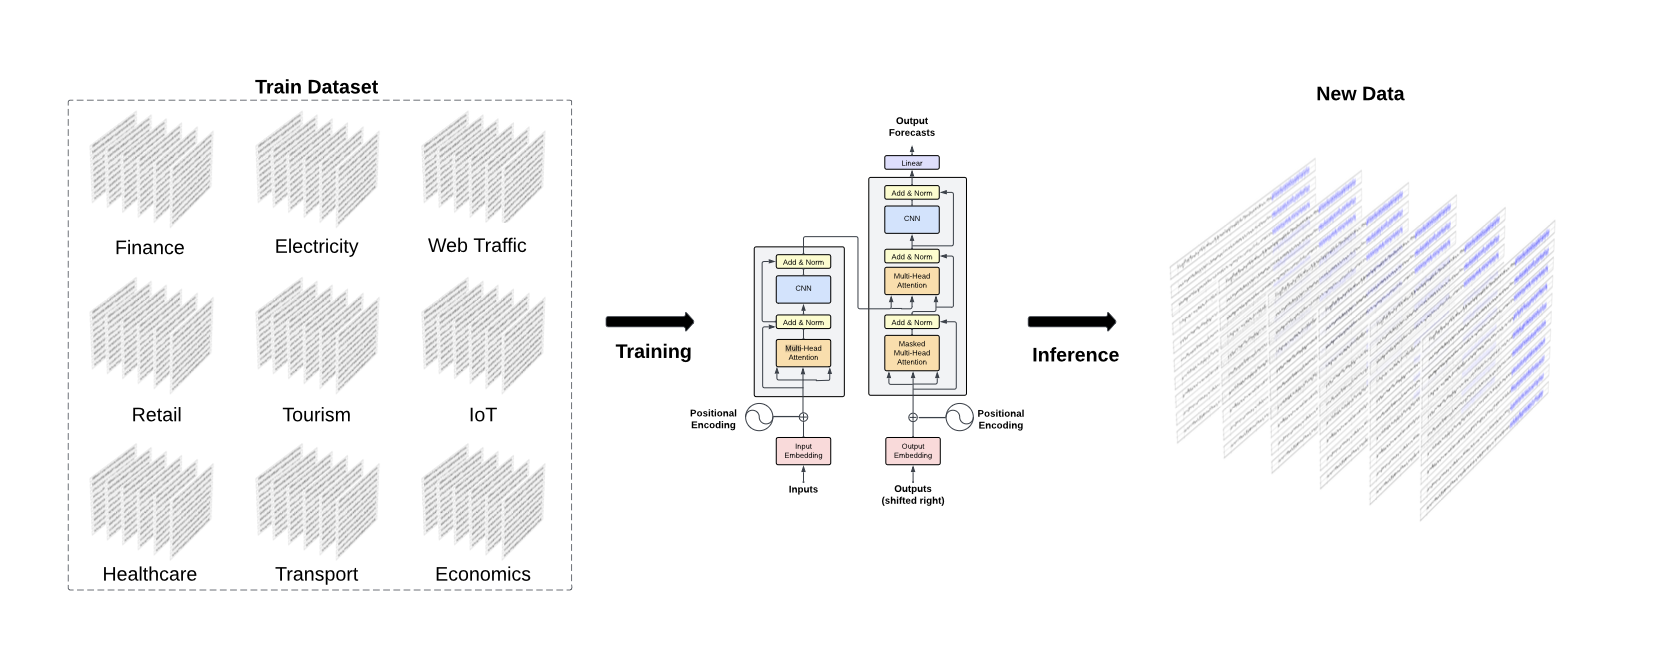
\includegraphics[width=1\linewidth]{images/foundation_model.png}
    \label{fig:mesh1}
    \caption{TimeGPT was trained in the largest collection of publicly available time series, and can
forecast unseen time series without re-training its parameters.}
\end{figure}
\\

\newpage
\subsubsection{Architecture and Training}
TimeGPT is built on the Transformer-based architecture with self-attention mechanisms. It uses historical data and makes a forecast ,while adding local positional encoding.The model can process different historical value windows and forecasting horizons, set by the user. The architecture consists of an encoder-decoder structure with multiple layers, with residual connections and normalization between all layers. The transformer-based architecture is the one that offers this high adaptability to TimeGPT model. Although this architecture uses the same principles as large language models (LLMs), TimeGPT is not based on an existing LLM.\\
\\
TimeGPT was trained on over 100 bilion data points, or as the authors say, the largest collection of publicly available time series to their knowledge. This collection includes datasets for a varied range of domains like finance, economics, demographics, healthcare, weather, IoT sensor data, energy, web, traffic, sales, transport and banking. 

\begin{figure}[h]
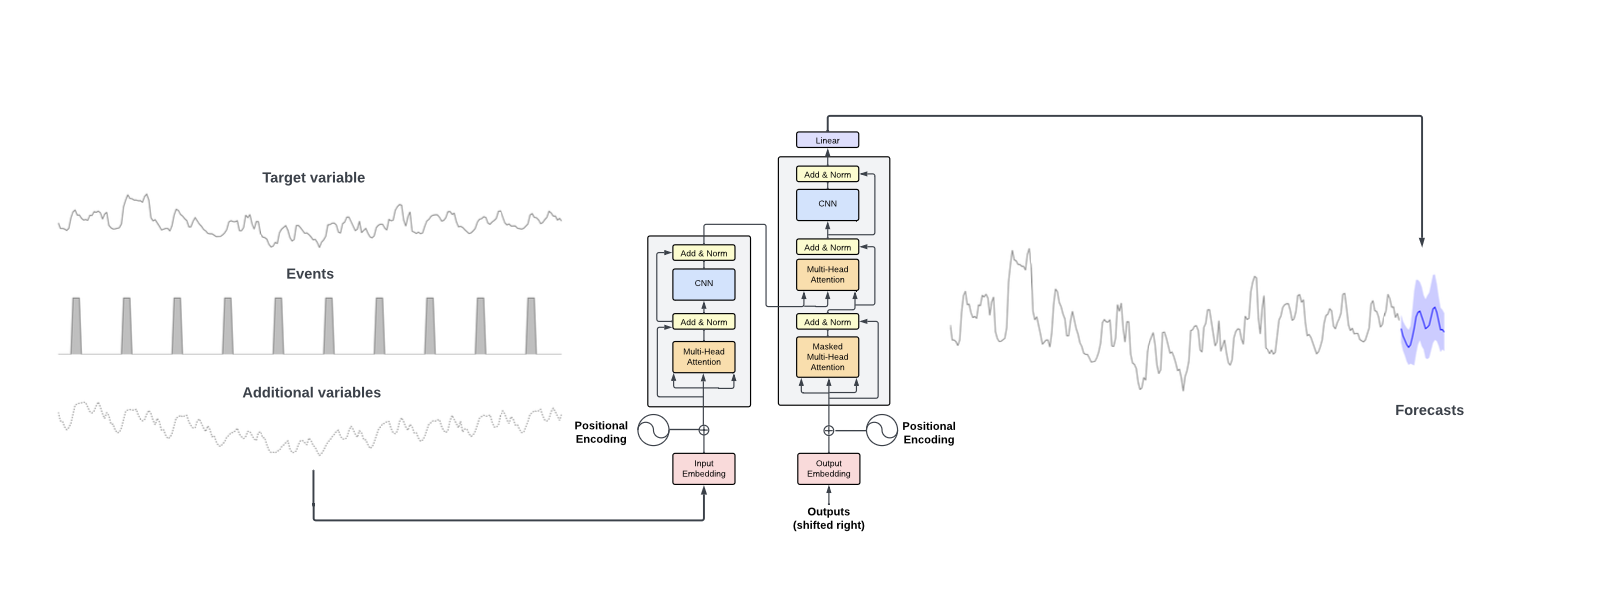
\includegraphics[width=1\linewidth]{images/timegpt_prediction.png}
    \label{fig:mesh1}
    \caption{Inference of new time series. TimeGPT takes the historical values of the target values and
additional exogenous variables as inputs to produce the forecasts. We rely on conformal predictions
based on historic errors to estimate prediction intervals.}
\end{figure}

\newpage
\subsubsection{Performance}
TimeGPT has demonstrated state-of-the-art performance across a wide range of benchmarks. According to the authors, it outperforms both classical baselines and deep learning methods on multiple datasets.\\
\\
In just zero-shot settings, TimeGPT consistently achieved lower forecasting errors, particularly in long-horizon forecasting, where traditional models often degrade. In particular, the model generalizes well to unseen datasets, suggesting that its pretraining objective captures domain temporal features.\\
\\
Moreover, TimeGPT supports fine-tuning, allowing it to adapt to new datasets with minimal supervision. These can decrease the forecasting error with an easy and flexible way, making TimeGPTs better, even in daily or hourly frequencies where models like NHITS and LGBM accordingly, showed lower error than TimeGPT.

\subsubsection{Advantages and Limitations}
The key advantages of TimeGPT include:

\begin{itemize}
    \item Scalability and generalization across domains and time scales.
\end{itemize}

\begin{itemize}
    \item Reduced reliance on labeled data and feature engineering.
\end{itemize}

\begin{itemize}
    \item High accuracy in long-range forecasting.
\end{itemize}

\begin{itemize}
    \item Strong zero-shot and fine-tuning capabilities.
\end{itemize}

\begin{itemize}
    \item Simplicity in usage.
\end{itemize}

\begin{itemize}
    \item Low time cost, capable for scalability.
\end{itemize}

However, it functions as a "black box", offering lower flexibility than statistical models or custom neural networks.


\subsection{Chronos Time-LLM}
Chronos is a foundation model for time series forecasting that uses Large Language models (LLMs) like T5 and GPT-2, to forecast time series through the novel yet simple idea of treating time series values as language tokens. Chronos uses the architecture of decoders-only transformers, similar to GPT models, but adapts the input format and  tokenization to process numerical and temporal information insted of text sequences.

\subsubsection{Architecture and Training}
Chronos includes a collection of LLMs, pre-trained on hundreds of time series datasets from a diverse range of application domains. Unlike other models Chronos handles time series data as a language-like stream of values Input sequences are tokenized and formatted as prompts, with numeric values treated as tokens and time information encoded through context windows \cite{ansari2024chronos}.\\
\\
Chronos Time-LLM model makes next-step predictions, using masked values and sliding windows during pretraining. It uses no explicit inductive bias for seasonality, periodicity, or stationarity -relying just on the generalization of large transformer decoders and transfer learning.\\
\\
The model is provided a small historical window of data, and it continues the sequence by predicting the future values. This ,like TimeGPT model, enables zero-shot and few-shot forecasting without fine-tuning or additional training, making the pretrained model able to be reused of varius tasks.

\subsubsection{Performance}
Chronos Time-LLM model was evaluated for both its in-domain and zero-shot generalization. It was compared with classic sstatistical models like ARIMA, ETS, Theta and with pretained LLM-based models like (PromptCast, LLMTime. GPT4TS, Time-LLM).\\
\\
When evaluated on datasets that Chronos was trained on, it outperformed all classical and deep learning baselines on the majority of tasks. Even smaller variants of Chronos like Chronos-S beat large models like PatchTST and DeepAR. It even outperformed models like GPT4TS and Time-LLM, which require tast-specific fine-tuning.\\
\\
Moreover, on datasets unseen during training from Chronos model used it's zero-shot generalization and was near or exceeded deep learning models trained on the specific dataset (PatchTST,TFT) and LLM-based models like LLMTime and PropmptCast that require engineered promprts.\\
\\
However, one of the key findings of this thesis is that the forecasting accuracy of Chronos deteriorates significantly beyond 64 time steps, due to the model’s reliance on a fixed input context window. Unlike TimeGPT, which supports long-horizon forecasting via fine-tuning, Chronos relies purely on pattern continuation, making it more suitable for short to moderate forecasting horizons.

\subsubsection{Strenghts and Limitations}
Chronos shows several strenghts for time series forecasting, like:

\begin{itemize}
    \item Prompt-based inference through in-context learning.
\end{itemize}

\begin{itemize}
    \item No need for model retraining or labeled supervision.
\end{itemize}

\begin{itemize}
    \item Generalization across domains due to pretraining on diverse time series.
\end{itemize}

However, it also has limitations like:

\begin{itemize}
    \item Performance degrades on very long or multivariate sequences compared to fine-tuned models like TimeGPT.
\end{itemize}

While Chronos shows strong results in settings where rapid, general-purpose forecasting is needed, it currently lacks the long-range robustness and tuning flexibility of more specialized models.

\subsection{Summary}
\subsubsection{Machine Learning Models}
Machine learning models like XGBoost, Support Vector Regression, and Random Forests had higher predictive performance than classical models, by using nonlinear modeling, nevertheless these models lack temporal awarness and requiring feature engineering to capture temporal patterns.

\subsubsection{Deep Learning Models}
Deep learning methods like LSTM networks, needs long training with large datasets to capture long-term temporal patterns. Are computationally expensive during training and also need feature engineering and achitectural fine-tuning. But with the right dataset and fine-tuning, LSTM's can have good results.

\subsubsection{Transformer and Foundation Models}
The most recent researches found are focused on foundation models for time series, including TimeGPT and Chronos Time-LLM. TimeGPT shows the power of fine-tuned, pre-trained models on varius datasets and long-range forecasting, while Chronos introduces a novel use of leanring via prompt-based inference. These models ,and specially TimeGPT, shows a new way for time series forecasting with simplicity, no training using its zero-shot capabilities, and flexibility with fine-tuning, one-hot
features and exogenous variables.

\section{Dataset Description and Preprocessing}
\subsection{Data Source and Features}
The data source for the dataset that was used in my thesis came from a retail company. It contains data collected in one of the company stores from 2023 to today.\\
\\
The data set consists of the number of visitors that entered and exited the store at a specific hour, and also the date and time.\\
In order to get the number of visitors that were inside the store each hour, I used the formula below assuming that:
\begin{itemize}
    \item  The visitors that entered the store are 'IN'
\end{itemize}
\begin{itemize}
    \item The visitors exited the store are 'OUT'
\end{itemize}
\begin{itemize}
    \item and hour is 't'
\end{itemize}
\\
Firstly, I calculated the Net Flow for each hour:
\begin{equation}
NetFlow = IN[t] - OUT[t]
\end{equation}
Then I calculate the number of visitors inside the store foe every hour:
\begin{equation}
Visitors = IN[t] + NetFlow[t-1]
\end{equation}
Net flow is used to help count the visitors that entered the store the previous hour but remained inside the store after the previous hour ended. This is a more accurate metric of true visitors in store per hour ,than just the visitors that entered that hour, and the one used for this thesis.

\subsection{Handling Missing Data and Outliers}
The original dataset included records only for the hours that the store was open ,specifically from 09:00 to 21:00, resulting in 12 observations per day rather than a full 24-hour sequence. However, the Time-GPT model requires a consistent time index to function properly. To fix that, I created additional rows to the non-operational hours (from 00:00 to 08:00 and from 22:00 to 23:00) for each day, ensuring consistency in the \texttt{datetime} column.\\
But this lead to missing values were created in the \texttt{visitors} column for the newly added time slots. Since the store was closed during these hours and no visitors could be present, I filled these missing values with zeros. This approach assured the continuity of the \texttt{datetime} column as required from Time-GPT model and kept the working hours of the store unchanged.

\subsection{Feature Engineering}
To help the models better capture temporal patterns and the seasonalities in the data, such as daily weekly, and monthly cycles, I added several time-related features. Specifically, I extracted the hour of the day, day of the week, calendar week, day of monthn, and month from the \texttt{datetime} column.
\\
The way to handle these features varied for each model. For the LSTM model I created
new columns for these temporal features and icluded them as additional inputs to the network. This allowed the model to learn patterns associated with specific time segments, like higher visitors during certain hours or days.\\
\\
For the other two models, Time-GPT and Chronos Time-LLM, it wan not necessary to add these features as column. Both models support one-hot encoding for time-based features, which enhances their ability to generalize temporal relationships across diiferen series and even domains.

\subsection{Data Splitting and Normalization}
For the LSTM model, I split the dataset into two parts: 75 percent was used for training and the remaining 25 percent for testing. Prior to training, I standardized the features to improve model performance and ensure numerical stability. The standardization was applied using the formula:

\begin{equation}
    Standardized Dataset = (dataset - mean) / std
\end{equation}

where the mean and standard deviation were calculated only from the training set to prevent data leakage.\\
\\
In contrast, both Time-GPT and Chronos Time-LLM are pre-trained models that do not require traditional training pipelines. As a result, I did not apply any train-test split or normalization when using these models, since they are designed to operate directly on raw input data and internally handle temporal patterns without additional preprocessing.

\newpage
\section{Implementation}
\subsection{Software and Tools Used}

To implement and evaluate the time series forecasting models in this thesis, I utilized a combination of programming languages, libraries, and cloud-based services. These tools enabled me to perform data preprocessing, model training, forecasting, and evaluation efficiently.
The entire implementation was in Python and made of use libraries like Pandas, Numpy, Matplotlib and Seaborn. Also used Tensorflow/Keras to train and predict with the LSTM model. At last, I accessed Nixtlas API for Time-GPT model and installed Chronos Time-LLM pretrained model.


\subsection{LSTM Model}
The LSTM model architecture and training approach were adapted from examples presented in the course lecture by Professor P.Louridas and from Deep Learning with Python (2nd Edition) by François Chollet \cite{Francois}. \\
\\
LSTMs are type of recurrent neural netwoks (RNN), specifically designed to capture long-term dependencies and sequencial patterns, making them well-suited for time series predictions tasks.

\subsubsection{Model Architecture}
The LSTM model was designed for multivariate predictions that takes as input historical data for the visitor counts (along with the other time features) and predicts the next 72 values in the series. Since the data are in hour level 72 value predictions, means 6 $days$ (= 72 $PredictionHours$ / 12 $HoursStoreIsOpen$). This prediction window and hours in the dataset was chosen to avoid having to predict Sundays and hours that the store is closed.

The architecture included:

\begin{itemize}
    \item One LSTM layer with 64 hidden units
\end{itemize}

\begin{itemize}
    \item A dropout layer to prevent early overfitting
\end{itemize}

\begin{itemize}
    \item A second LSTM layer with 32 hidden units
\end{itemize}

\begin{itemize}
    \item A second dropout layer to prevent overfitting
\end{itemize}

\begin{itemize}
    \item A fully connected (dense) output layer with 72 neurons responsible for forecasting the next 72 values.
\end{itemize}


 \subsubsection{Data Preparation and Input Shaping}
To prepare the data for the model, first additional features had to be created.This features as mensioned before are temporal values like hour, day of week, day of month and month. These additional features are used to help the model catch seasonality and temporal cycles within the dataset.\\
\\
To train the LSTM neural network, sliding windows were created. Each input included a window of previous time steps and the corresponding target was the visitors count for the next time step (hour). The dataset was split into 75 percent training and 25 percent testing sets, and all in iput features were standardized using the men and standard deviation of the training dataset.

\subsubsection{Training Configuration}
The model was compiled using Adam optimizer and the Mean Absolute Error (MAE) as the loss function. The training was performed for 50 epochs with a batch size of 256. Early stopping was also applied on the validation loss to prevent overfitting.\\
\\
The hyperparameters such as window size, hidden units per layer, dropout rate, and learnign rate were tuned experimentally and manual changed to better the evaluation on the validation set and opitize the loss function.\\
\\
The loss functions for the training can be seen below:

\begin{figure}[h]
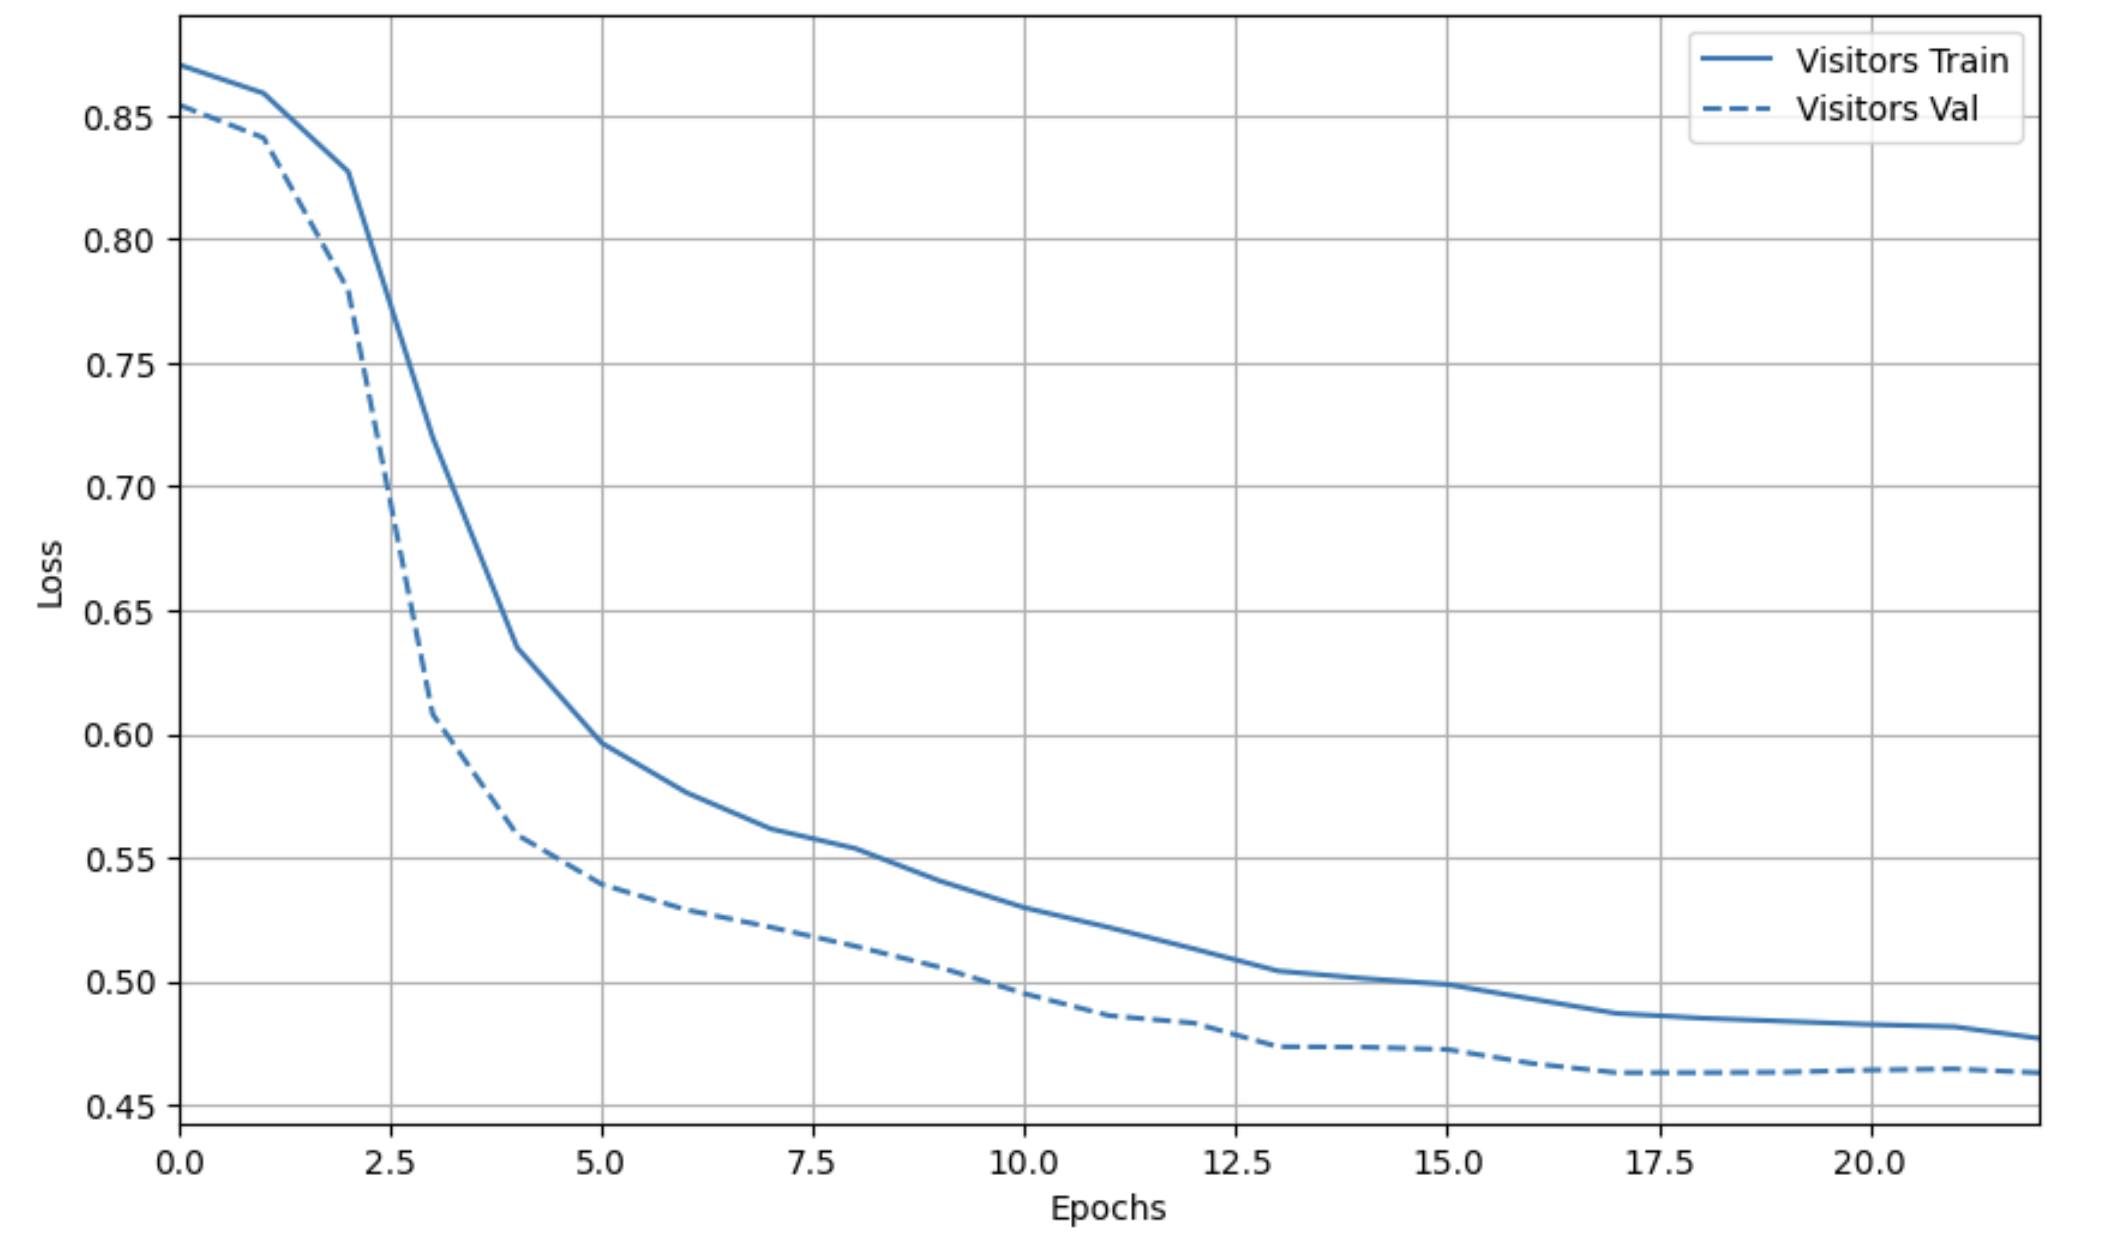
\includegraphics[width=1\linewidth]{images/loss_function.png}
    \label{fig:mesh1}
    \caption{Loss Function}
\end{figure}

\subsubsection{Forecasting Procedure}
After the training, the model was used to make a forecast on the test dataset using the rolling window approach. At each step, the model predicted the next time point based  on the most recent sequence of observations. Then the predictions were compared with the ground truth values to make an evaluation for the perfomance of the models forecast, using the Mean Absolute Error (MAE). \\
\\
The model proved to be a valuabled baseline to compare against the newer and most advansted Time-GPT and Time-LLM models, providing usefull insights into the benefits of Deep Learning against more transormer-based approaches.

\begin{figure}[h]
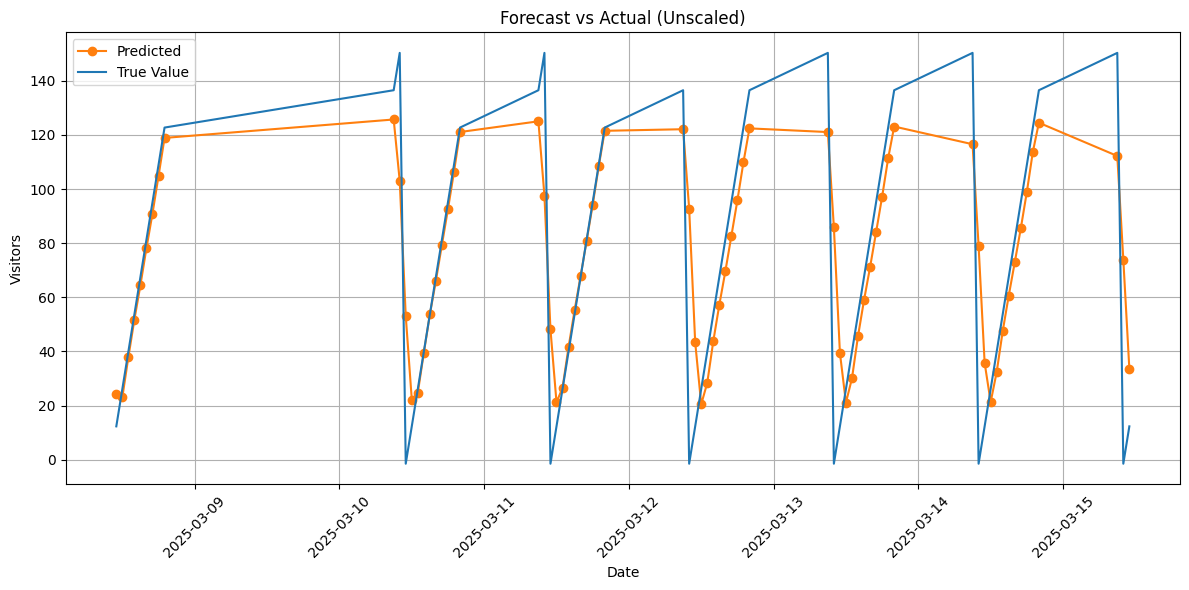
\includegraphics[width=1\linewidth]{images/neural_forecast.png}
    \label{fig:mesh1}
    \caption{LSTM Neural Network Forecast}
\end{figure}

\newpage
\subsection{Time-GPT Model}
Time-GPT is a time series forecast  model developed by Nixtla, which is 
pre-trained for large-scale predictions. It has a Transformer-based architecture with self-attention mechanisms. Time-GPT's architecture make it highly adaptable in varied frequencies and characteristics while even been able to process different input sizes and forecasting horizons \cite{garza2024timegpt1}. Also, as the authors say the zero – shot inference Time-GPT provides, proves to excel at performance, efficiency and simplicity.\\
\\
In this section, the reader is informed about the process of integrating Time-GPT into the forecasting pipeline, including the model’s configuration, input formatting, and inference procedure on the retail visitors dataset.


\subsubsection{Model Overview and Access}
Time-GPT can be accessed as a hosted API service via Nixtla’s cloud platform, which enables easy deployment and prediction without the need for local model training. For this study, the timegpt-1-long-horizon endpoint was used, a general-purpose model pre-trained on a wide variety of time series domains, best suited for long-term forecasting.\\
\\
Access to the model was established using Nixtla’s Python client, and forecasts were generated via REST API calls. This approach provided a low-overhead and scalable method for experimentation, especially for zero-shot forecasting scenarios.


\subsubsection{Data Preparation and Input Formatting}
To generate forecasts using Time-GPT, input data must be structured as a Pandas DataFrame containing at minimum the following fields:\\
\\
•	ds: The datetime values of the historical series.\\
•	y: The corresponding numerical values (i.e., hourly visitors).\\
•	unique-id: An identifier for each time series (in this case, a single ID was used for the entire dataset).\\
\\
Additionally, I specified the forecasting horizon (h) to match the future time window I aimed to predict, and used a window of  168 hours (= 7 * 24)  meaning a week. I also created two new one - hot columns ('is-sunday' and 'store-closed') for the model to understand the days that are Sundays when the store is usualy closed and if it is actually closed since there are Sundays that the store remains open like the weeks of December before Christmas. These two columns are used a future exogenous variables to provide more information the model about future events in order to predict accurately during known events that are going to happen.\\
\\
Moreover the model was finetuned using the Mean Absolute Error as the loss function of the model and also made of use the date features provided by Nixtla in there models as an option. These features were ('dayofyear','dayofweek','month', 'day','week','year', 'hour') which are one – hot features that help the model understand patterns that appear through the dates when they happen multiple times.\\
\\
Normalization was not applied to the input values since the model could predict with high performance using just the true values of visitors from my dataset.\\


\subsubsection{Forecasting Procedure}
Forecasts were generated in a rolling-window fashion. For each evaluation segment, the model was queried using the latest available historical values and instructed to predict the next (h) steps. The results were returned in the form of a dataframe of the predicted values with associated timestamps, enabling direct alignment with ground-truth data for evaluation.
Since Time-GPT is pre-trained and does not require model training to be performed on the dataset. This makes it particularly suitable for real-time forecasting applications where retraining is infeasible or costly.\\


\subsubsection{Observations and Performance Considerations}
The use of Time-GPT introduced several practical benefits:\\
\\
•	Zero-Shot Capability: The model demonstrated competitive performance without fine-tuning, highlighting the strength of foundation models in forecasting.\\
•	Simplicity of Integration: The hosted API structure minimized the need for local infrastructure or deep model knowledge.\\
•	Strong Temporal Awareness: The model effectively captured daily and weekly seasonality patterns inherent in the dataset.\\
•	Exogenous Variables: The model supports the incorporation of additional variables to enhance forecast accuracy.\\
\\
However, some limitations were also observed:\\
\\
•	Limited Transparency: As with many black-box models, interpreting the logic behind predictions is non-trivial.\\
•	Dependency on API Access: Reliance on a hosted service presents concerns about latency, pricing, and offline accessibility.\\
\\
Despite these constraints, Time-GPT represents a robust and flexible solution for time series forecasting, and its integration served as a valuable benchmark in our comparative evaluation.

\begin{figure}[h]
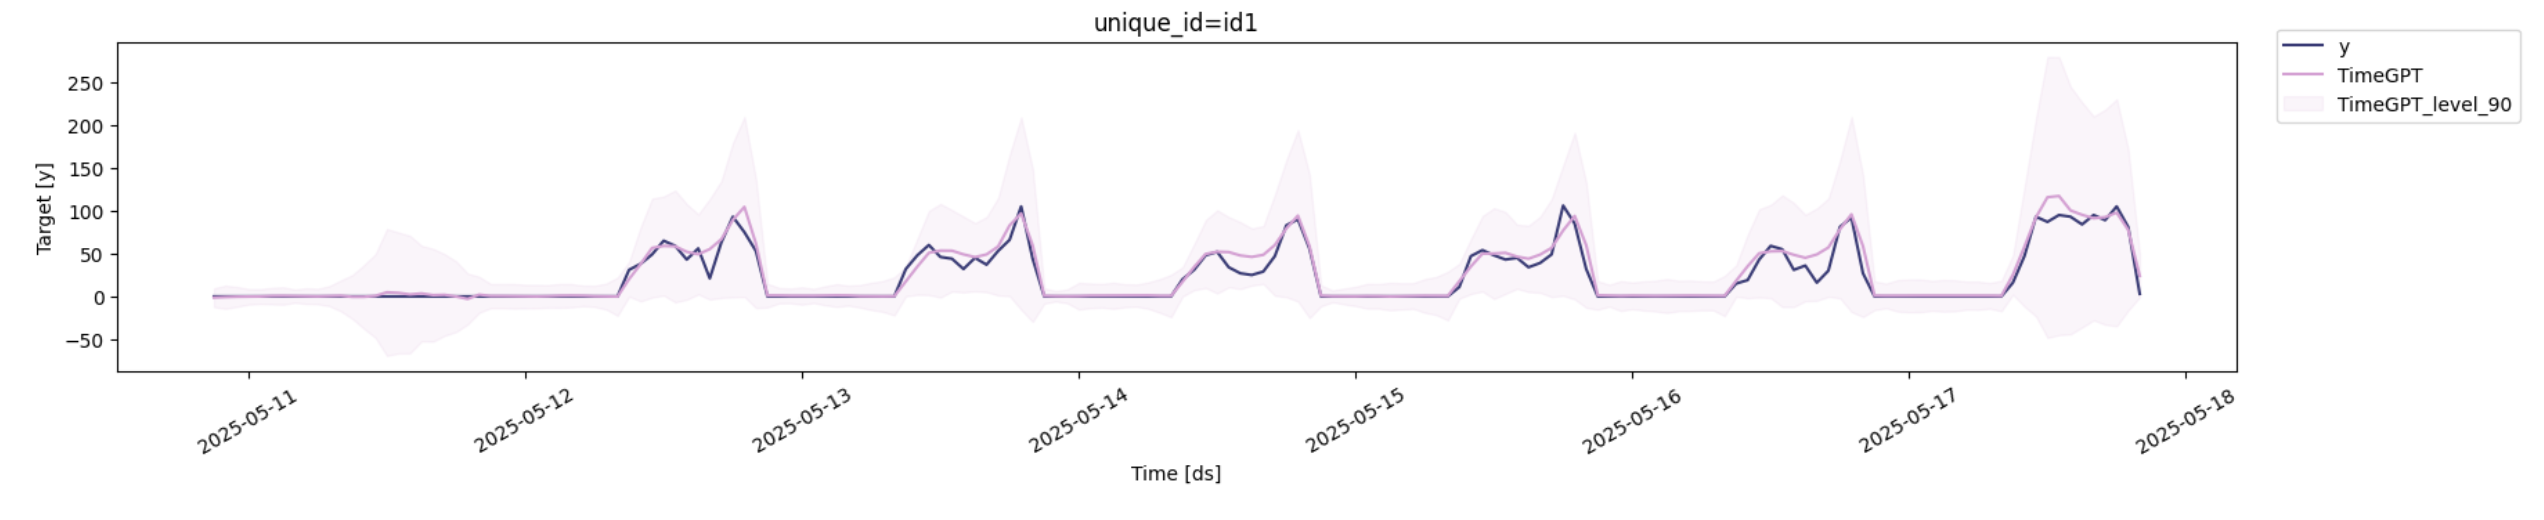
\includegraphics[width=1\linewidth]{images/timegpt_forecast.png}
    \label{fig:mesh1}
    \caption{Time-GPT Forecast}
\end{figure}


\subsection{Chronos Time-LLM}
Chronos is a time series forecasting framework developed by Amazon that integrates the capabilities of large language models (LLMs) with temporal data modeling. Unlike traditional neural networks or even general-purpose transformers, Chronos is specifically fine-tuned and pre-trained on a diverse set of time series datasets. In this section, I describe the process of implementing the Chronos Time-LLM model for my dataset, discuss its integration pipeline, and highlight the specific adaptations made to ensure compatibility with our retail visitors time series dataset.\\

\subsubsection{Model Selection and Configuration}
The Chronos framework offers several pre-trained checkpoints, each one optimized for different forecast horizons. For this thesis, the general-purpose chronos-t5-base model was selected due to its strong performance across a wide variety of datasets in prior evaluations as the authors and creators of the model has sawn. The zero-shot setting allows for evaluating the model’s generalization capability without domain-specific fine-tuning, which makes it a highly applicable pre-trained Time-LLM.

\subsubsection{Forecast Generation}
For each test sample, the Chronos model generated a multi-step forecast using a rolling window approach. That means, predictions were made for a defined horizon of 64 hours into the future, and the forecast window advanced incremental to cover the full evaluation period.\\
\\
These forecasts were then aggregated and used for comparison against the LSTM and Time-GPT models, as detailed in Chapter 7.

\subsubsection{Limitations and Observations}
While Chronos Time-LLM demonstrated strong generalization and required minimal training effort, it presented several practical challenges:\\
\\
•	Forecast Latency: Forecast generation was slower compared to Time-GPT model, especially when using large context windows.\\
•	Hidden Internal Mechanisms: Due to its LLM-based architecture, understanding how the model derives its forecasts is less transparent compared to standard deep learning models.\\
\\
Nevertheless, its ability to produce accurate forecasts without task-specific tuning represents a major advancement in the field of time series forecasting.


\begin{figure}[h]
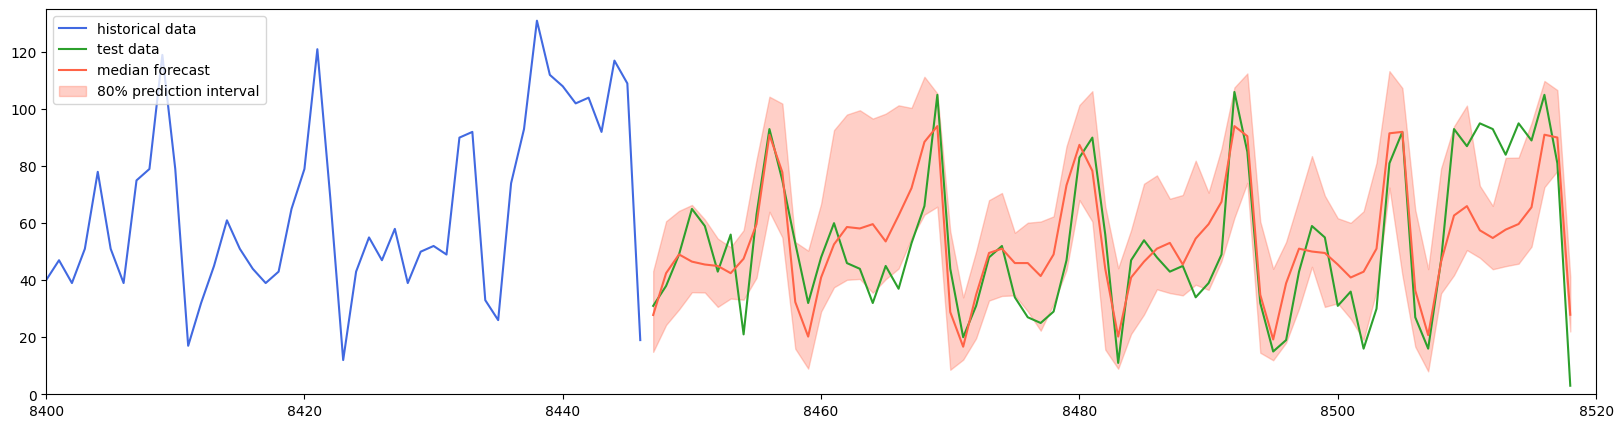
\includegraphics[width=1\linewidth]{images/chronos_forecast.png}
    \label{fig:mesh1}
    \caption{Chronos Forecast}
\end{figure}


\section{Results and Evaluation}
In this chapter, the results of the evaluations are been presented and compared for the models implemented in this thesis: LSTM, Time-GPT and Chronos Time-LLM. I evaluate, and discuss the specific strengths, weaknesses, and best-use scenarios for each approach.

\subsection{Forecasting Performance}
Time-GPT demonstrated the strongest overall performance, particularly in forecasting in longer horizons. It consistently had accurate predictions even in long miltistep predictions. In contrast, Chronos Time-LLM showed a noticeable drop in precision after the 64th forecasting step, which is a known limitation of its architecture -for the $chronos-t5-base$ model at least. Even within this limit, Chronos showed a higher Mean Absolute Error (MAE) compared to Time-GPT, indicating less stable short-term performance. \\
\\
The LSTM model, trained sprecifically on the dataset, captured general temporal trends and was better than the transormer-based model,Chronos, in accuracy. It offered flexibility and full control over the model design and training process. The experimentation for the optimal layers, hidden units and dropout layers alongside with the additional temporal features gave the edge to the LSTM model.\\
If Chronos Time-LLM model was better finetuned and one-hot encoding was used it might got a closer MAE as the LSTM model's or even lower.\\
\\
These observations highlight that Time-GPT is better suited dor applications requiring longer Forecasting windows and minimal training effort. There is a big gap between Time-GPT and the other two models. The LSTM model comes second and Chronos with a relatively small difference but both are promising in getting better with more features and finetuning.\\
\\
Although, LSTM model has high flexibility and complete control even in training both pretrained models support finetuning and exogenous variables (features).\\
Chronos model lacks in long horizon forecasting since any more than 64 steps, is not even recommended by the authors.


\subsection{Quantitative Analysis}
%%%%%%%%%%%%%%%%%%%%%%%%%%%%%%%%%%%%%%%%%%%%%%%%%%%%%%%%%%%
\begin{itemize}
    \item Mean Absolute Error (MAE)
\end{itemize}

\begin{table}[h]
\centering
\begin{tabular}{|c|c|c|}
\hline  
\textbf{Model} & \textbf{MAE} \\
\hline
LSTM Neural Network  & 15.70 \\
\hline
Time-GPT Tuned  & 5.08 \\
\hline
Time-GPT Not Tuned &  9.49 \\
\hline
Chronos Time-LLM  & 18.18 \\
\hline

\end{tabular}
\caption{Model Comparison}
\label{tab:example}
\end{table}
%%%%%%%%%%%%%%%%%%%%%%%%%%%%%%%%%%%%%%%%%%%%%%%%%%%%%%%%%%%

Time-GPT outperformed the other two models. LSTM model ranked second but remained highly less precise than Time-GPT, while Chronos Time-LLM model showed slightly higher error rates than LSTM model, and the higher of them all, particularly in scenarios of longer prediction windows.

\subsection{Visual Comparison of Forecasts}
To complement the numerical evaluation, I plotted the predicted values from each model against the actual visitor counts.

\begin{itemize}
    \item \textbf{LSTM}: Forecast were generally good but missed higher and lower values.
\end{itemize}

\begin{itemize}
    \item \textbf{Time-GPT}: Captured trends and seasonality after using one-hot features, exogenous and future exogenous variables.
\end{itemize}

\begin{itemize}
    \item \textbf{Chronos Time-LLM}: Was on the right track but often missed lower values. Better finetuning could result to higher accuracy.
\end{itemize}

\subsubsection*{A closer look at the Visual Comparison Forecasts}
As we compare Time-GPT finetuned and Chronos Time-LLM models, we can see that both models tend to capture the temporal sequence well enough and not decline an lot from the ground truth values for the most part of the prediction. The models miss some values in the same hours. Having a closer look it proved that these hours that both models miss the visitors count are the middle of the day and this sudden drop of visitors is hard to predict. However, Time-GPT when finetuned predicts closer to the true value than Chronos. That means that captures trends better.

 \begin{figure}[h]
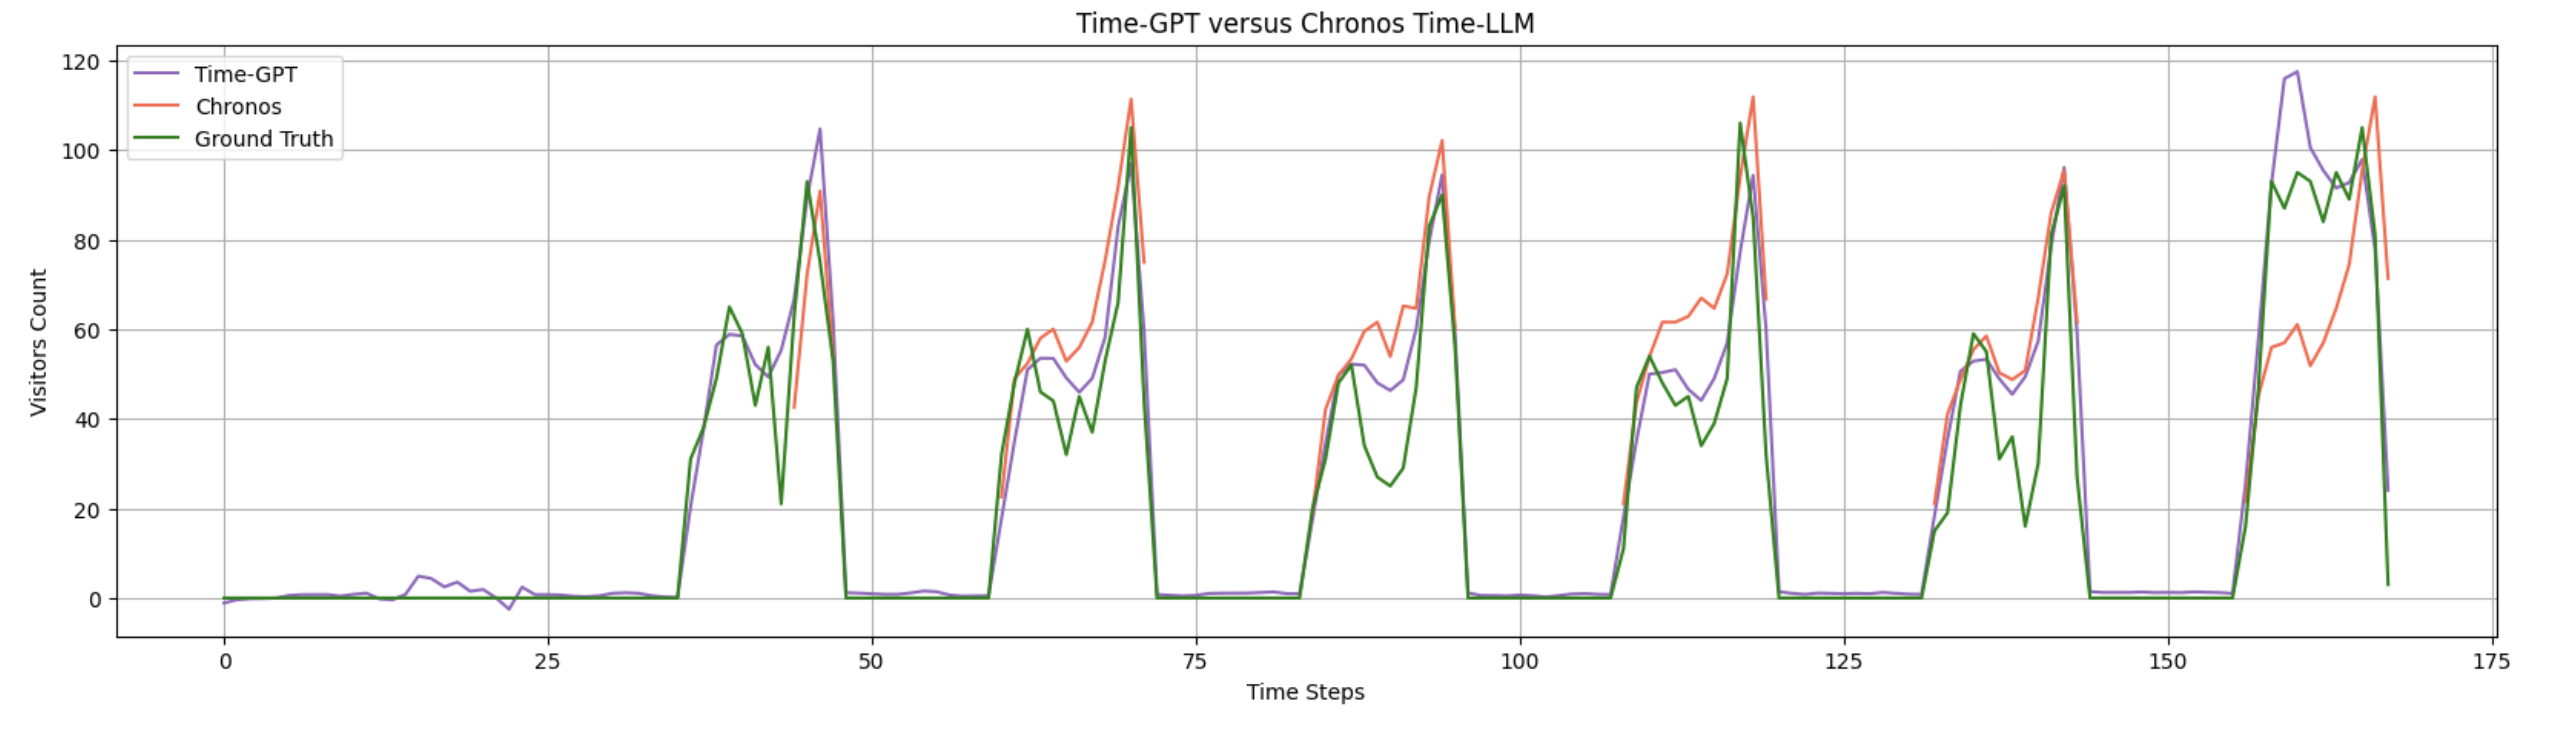
\includegraphics[width=1\linewidth]{images/TimeGPT_versus_Chronos_Forecast.png}
    \label{fig:mesh1}
    \caption{Time-GPT versus Chronos Time-LLM}
\end{figure}

It is interesting to see the difference that finetuning makes to the Time-GPT model.\\
\\
As said before, \textbf{Time-GPT finetuned} has a MAE of \textbf{5.08} while \textbf{non finetuned} a MAE of \textbf{9.49}. That a relatively small difference. Visually comparing the two models, one can notice two things. Firstly, their temporal sequences shows similarities but the finetuned model gets closed to the ground truth values. Secondly, there are gaps between the days and also in the start of the prediction an empty space appears ,that no true visitors were counted. The gaps represent the hours that the store is closed, the empty space is a $Sunday$ where the store is also closed. The same happens on holidays -stores are closed. The finetuned model is able to capture these 'special' occasions almost perfectly while the non tuned model is unaware of $Sundays$ and holidays, but is not so bad identifying the gaps between days especially in the later part of the prediction.\\
\\
This can show the significance of finetuning Time-GPT and the power and flexibility it has, to be customized upon a specific dataset even though it uses zero-shot forecasting, meaning that it is not trained of the exact dataset.\\
This also proves that even non tuned Time-GPT is well trained and can easily capture the temporal sequence of every dataset it used upon.

\begin{figure}[h]
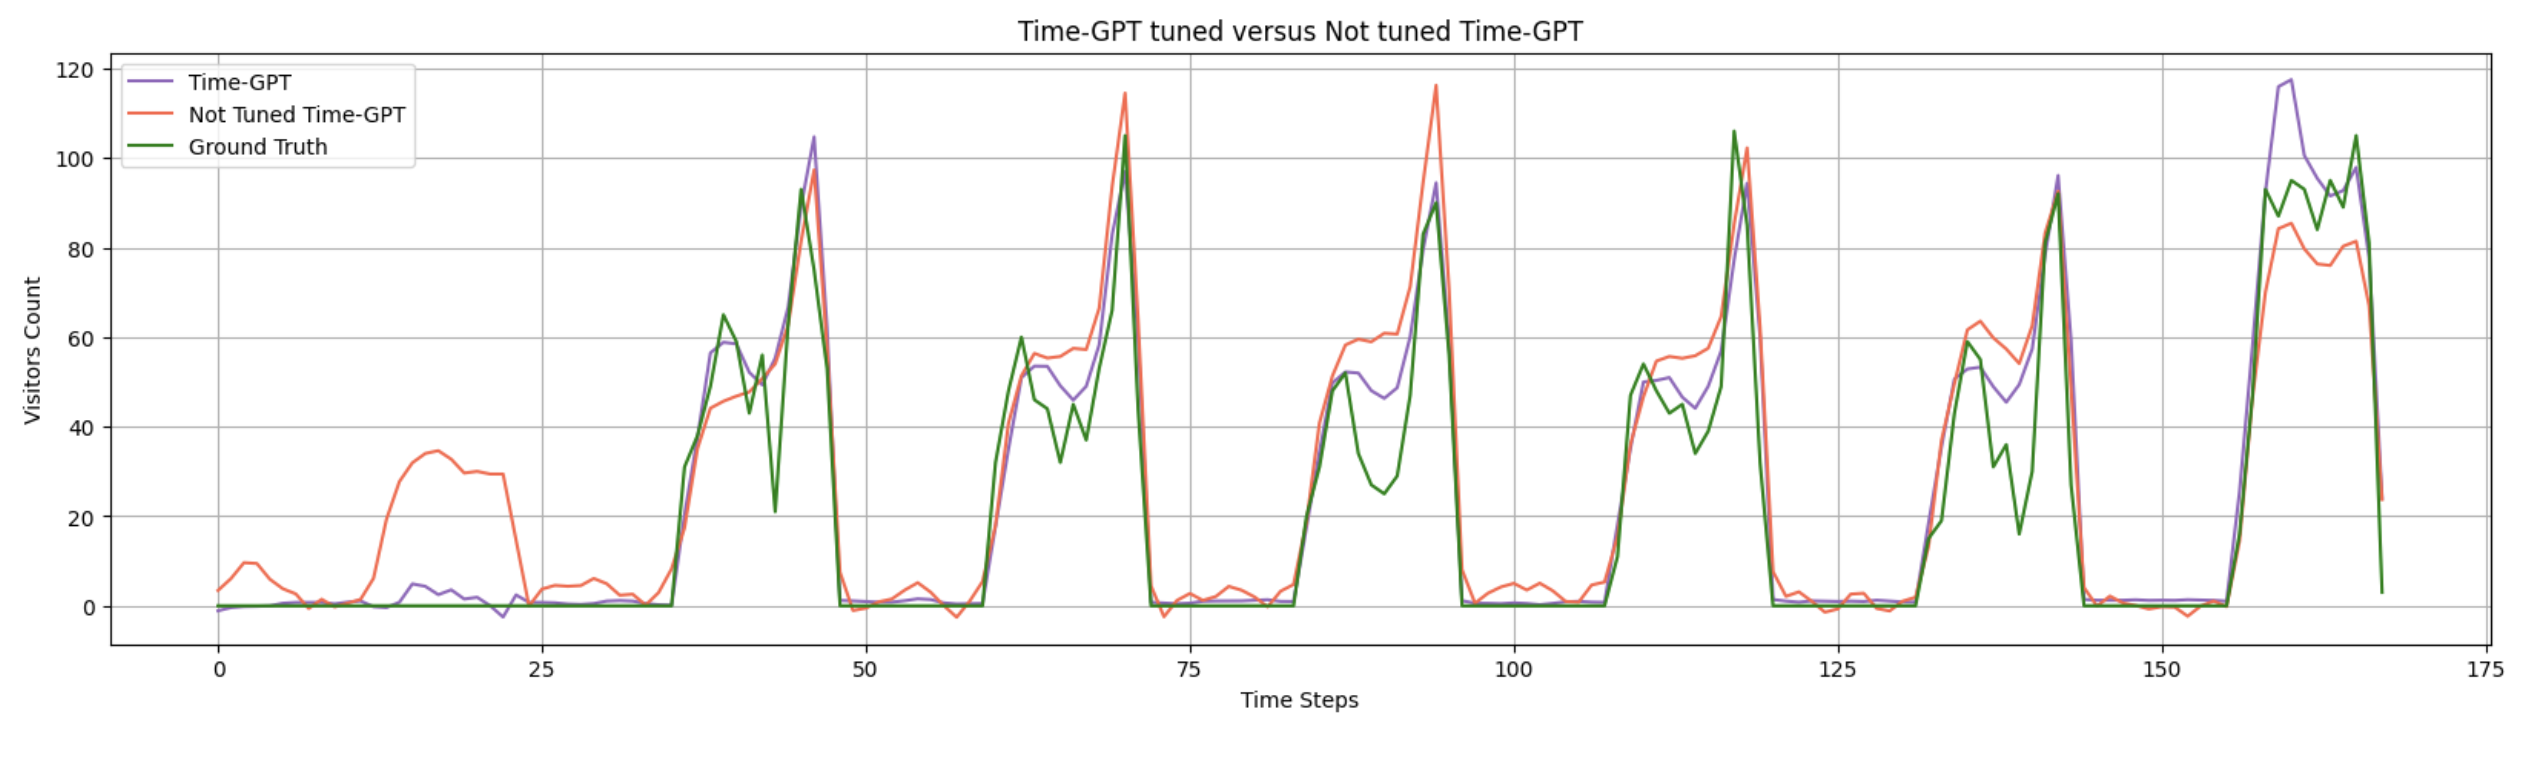
\includegraphics[width=1\linewidth]{images/TimeGPT_Tuned_and_Not_Forecast.png}
    \label{fig:mesh1}
    \caption{Time-GPT finetuned versus Time-GPT not finetuned Forecast}
\end{figure}

At last, LSTM neural network model captures most of the values very well but it lacks during the very high and low values and this rises its MAE.

\begin{figure}[h]
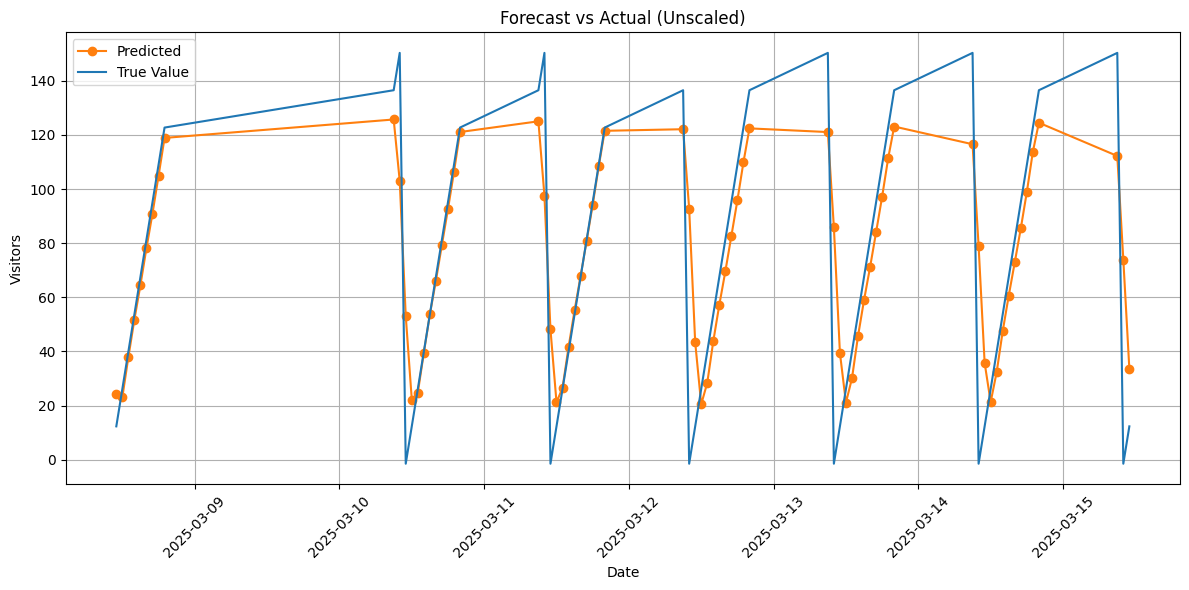
\includegraphics[width=1\linewidth]{images/neural_forecast.png}
    \label{fig:mesh1}
    \caption{LSTM model Forecast}
\end{figure}
\newpage
\subsection{Discussion of Results}
 The evaluation results clearly highlight the strenghts and weaknesses of each forecasting model. Among all models tested, the \textbf{Time-GPT (tuned)} version achived the best performance, with a \textbf{Mean Absolute Error (MAE) of 5.08}. This demonstrates the effectivness of fine-tunning Time-GPT for the specific structure and behavior of the dataset. Its ability to adapt to temporal patterns and fluctuations in visitors traffic led to highly accurate forecasts.\\
 \\
 The non-tuned version of Time-GPT, also performed weel, achieving a MAE of 9.49. While slightly less accurate, it still outperformed both Chronos and LSTM model, showing that even without customization, Time-GPT is capable of capturing well enough seasonal patterns in a zero-shot setting. This makes it a powerful tool under almost any circumstance.\\
 \\
 On the other hand, the Cronos Time-LLM model resulted in the \textbf{highest error}, with a MAE of 18.18. Although Chronos is designed for general-purpose time series forecasting, its performance degraded over long horizons. As noted in earlier sections, Chronos is limited to 64-step prediction windows, and after that its accuracy declines as it exceeds this threshold. Even within valid input ranges, Chronos tends to mainly over-estimate values. It is possible to lower the error of the model drastically by finetuning it. Overall it is a good predicting model that captures temporal patterns well enough with easy and quick implementation.\\
 \\
The LSTM neural network, with a MAE of 15.70, provided reasonable results considering its simplicity compared to the other models and the need for training. It captured the overall structure of daily visitors traffic but often missed the high and low values along with sudden changes or spikes.\\
Unlike the other two models, the LSTM requiers feature engineering, careful tuning, and more extensive preprocessing. However, it remains a useful option when full control over the modeling pipeline is needed.\\
\\
In summary:
\begin{itemize}
    \item \textbf{Time-GPT finetuned} offers the best accuracy and generalization.
\end{itemize}
\begin{itemize}
    \item \textbf{Time-GPT not finetuned} provides strong performance out of the box, useful for fast, zero-shot forecasting.
\end{itemize}
\begin{itemize}
    \item \textbf{Chronos Time-LLM} is more limited in forecasting range and overall precision but captures trends well.
\end{itemize}
\begin{itemize}
    \item LSTM is a viable baseline but lacks the accuracy of Time-GPT. However with the right features and finetuning could be improved.
\end{itemize}
 
 These findings emphasize the practical benefits of using large, pre-trained models for time series forecasting -particularly when ease of deployment and predictive performance are both critical.
 
\newpage
\bibliographystyle{plain}
\bibliography{references.bib}
\nocite{*}

\end{document}
